\documentclass[uplatex,a4j]{jsreport}
\usepackage{title}
\usepackage{thesis}
\usepackage[dvipdfm]{pict2e}
\usepackage{qtree}

\begin{document}
\title{HTML5字句解析仕様の\\自然言語処理による意味解析}
\author{五十嵐彩夏}
\studentid{17B01064}
\department{東京工業大学 情報理工学院 数理・計算科学系}
\supervisor{南出靖彦 教授}
\degree{学士}
\schoolyear{令和2年度}
\submitday{1月18日}

\maketitle

%\documentclass[uplatex,a4j]{jsreport}

\begin{document}
\begin{abstract}
  概要.概要.概要.概要.概要.
  がいよう
  % 序論の内容まとめる1/3ページ
\end{abstract}
\end{document}

\pagenumbering{roman}

\tableofcontents
\newpage

\pagenumbering{arabic}

%%% ここに各章をinclude %%%
\documentclass[uplatex,a4j]{jsreport}
\usepackage{thesis}

\begin{document}
\chapter{序論}

自然言語は, 人間が同士が互いにコミュニケーションをとるために発展してきた言語である.そして自然言語をコンピュータにで処理する技術を自然言語処理(Natural Language Processing)と呼んでいる.
本論文では自然言語処理の技術を使ってHTML5の字句解析仕様から命令を抽出することを試みた.

% html5の構文解析に関する研究の話 + どうしてやろうと思ったか
過去に行われてきたHTML5の構文解析の検証に関する研究には, XSS(クロスサイトスクリプティング)保護機構であるXSSAuditorのトランスデューサでのモデル化による有効性の検証~\cite{XSSAuditor} ~\cite{トランスデューサの包含関係}や, 
HTML5構文解析仕様の到達可能性の解析 ~\cite{HTML5Testing}などがある. 
それらの研究では実装の評価において, 自然言語によって書かれているHTML5字句解析仕様から, 命令を手作業で抽出している. 
よって構文解析の検証における実装の負担を減らすために, 仕様書からの命令の抽出,  形式化を自動化したいと考えた. 
さらに, 仕様の形式化の自動化が出来るようになることによって, 仕様の変更が行われる際, 仕様の定式化を自動化していれば, 変更への対応が楽になるというメリットもある.
% 仕様の変更が行われることがあるため, その時に仕様の定式化を自動化していると嬉しい.

% 一般的な仕様の定式化が出来るツールがあると嬉しい.

%ARMの研究の話
仕様書から自然言語処理を用いて命令抽出を試みた研究としては, 機械語命令ARMの仕様書を対象としたものがあり, 
そこでは, 自然言語処理の構文木解析などの結果を用いて, 命令の抽出を行っていた.~\cite{arm}\\

% 使用ライブラリ
実装では, 自然言語処理のライブラリとして, スタンフォード大学によって提供されている Stanford CoreNLP~\cite{manning-EtAl:2014:P14-5}を使用した.


%====何か書く==-
(何か書く)

図\ref{流れ}がHTML5の字句解析仕様の意味解析の概要である.\\
% 概要の図
\begin{figure}[h]
    \centering
    \includegraphics[keepaspectratio, scale=0.6]
         {figure/流れ2.png}
    \caption{流れ(仮)}
    \label{流れ}
\end{figure}
\\
% ここの部分を何章で説明する, とかを書く
本論文では, まず\ref{準備}章で自然言語処理の基礎知識を述べる.
次に\ref{字句解析仕様}章で HTML5 の字句解析器の主な仕様, 動作について述べる.
\ref{形式}章で抽出する命令の形式をBNFとして述べ, 
\ref{自然言語処理}章で自然言語処理ライブラリを用い, それをHTML5字句解析仕様に適用させ, 
\ref{命令抽出}章で自然言語処理の出力をもとに仕様書の命令の抽出を行った. 
\ref{実装}章で抽出した命令をもとに字句解析をするインタプリターを作成し, 
\ref{評価}章で字句解析のテストデータを用い, 抽出した命令の正しさを検証した.
\end{document}

\documentclass[uplatex,a4j]{jsreport}
\usepackage{thesis}

\begin{document}
\chapter{準備}
\label{準備}
% 読んでもらうことに必要なこと
% 自然言語処理のこと,必要な言葉
%html5のtokenerser仕様のこと
\section{品詞タグ}
% 自然言語処理のチャプターでやる
準備~\cite{pennTreebankTags}
S : 節
VP : 動詞句
NP : 名詞句
VB : 動詞

\section{自然言語処理}
\subsection{使用ライブラリ}
自然言語処理のライブラリとして,Stanford CoreNLP~\cite{manning-EtAl:2014:P14-5}を使用した.
Stanford CoreNLPは自然言語処理ツールのひとつであり,スタンフォード大学によって提供されている.
StanfordCoreNLPでは,
% ライブラリでどういう情報を得られるか
形態素解析(品詞タグ付け、単語の原型の取得),構文解析,意味解析などが出来る.\\
%以下の例で詳しく述べる.\\
% pipelineの説明をする===
(pipelineの説明をする)\\
%====
\subsection{概要}
"Mika likes her dog's name."をStanford CoreNLPで自然言語処理をさせる.
\subsubsection{トークン分割、品詞タグ付け、原型}
Mika/NNP  likes/VBZ her/PRP\$ dog/NN 's/POS name/NN ./.\\
Mika/Mika  likes/like her/she dog/dog 's/'s name/name ./.
\subsubsection{固有表現抽出}
数字や時間、アドレス、人間、地名といった固有な表現を抽出することが出来る.\\
Mika : PERSON
\subsubsection{構文木解析}
\Tree [.S [.NP [.NNP Mika ] ]
           [.VP
              [.VBZ likes ]
              [.NP [.NP [.PRP\$ her ][.NN dog ][.POS 's ] ]
                    [.NN name ] ]
           ]
           [.. . ]
      ]
\subsubsection{係り受け解析}
係り受け解析とは、単語間の関係を解析するものである.\\
\begin{figure}[h]
  \centering
  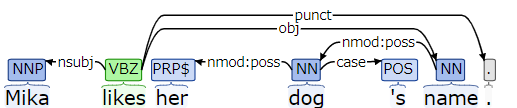
\includegraphics[keepaspectratio, scale=1.0]
       {figure/dependency.png}
  \caption{dependency}
  \label{dependency}
\end{figure}
\subsubsection{参照関係の解析}
参照関係の解析とは,文章内で複数個同じものを指し示す単語がある時、それを抽出するものである.itやheなどの指示語の指し示すものを見つける時になどに使用される.\\
Mika, her
\end{document}
\documentclass[uplatex,a4j]{jsreport}
\usepackage{thesis}

\begin{document}
\chapter{HTML5字句解析器}
\section{HTML5字句解析仕様書}
HTML5字句解析仕様はWHATWG communityのwebサイトから得られる.~\cite{html5specification}
HTML5の字句解析仕様には80個の状態がある.
\begin{figure}[h]
    \centering
    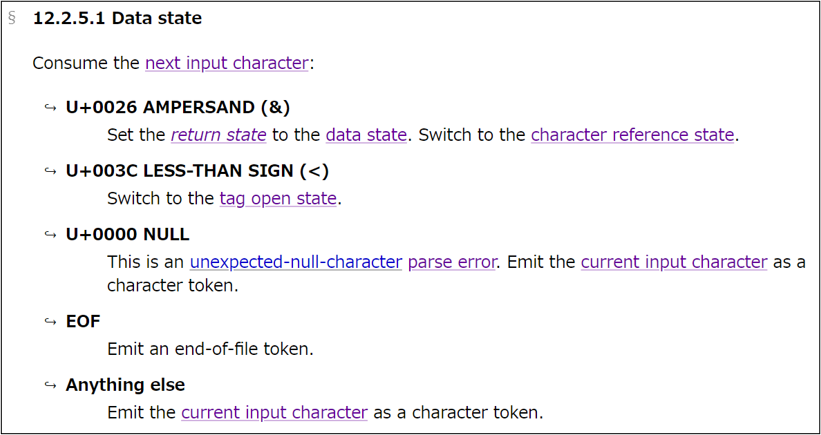
\includegraphics[keepaspectratio, scale=1.0]
         {figure/html5.png}
    \caption{HTML5字句解析仕様書}
    \label{html5}
\end{figure}
   aaa図\ref{html5}

%% BNF
\section{BNF}
$cList$ : CommandList\\
c : Command\\
b : Bool\\
cval : CommandValue\\
ival : InplementVariable\\
\begin{eqnarray*}
    {\rm cList }&\bnfdef& c :: cList \bnfor Nil\\
\end{eqnarray*}
\begin{eqnarray*}
    {\rm c }&::=& \mbox{if $\langle$Bool$\rangle$ then $\langle$cList$\rangle_1$ else $\langle$cList$\rangle_2$}\\
      &|& \mbox{ Ignore() //} \\
      &|& \mbox{ Switch($\langle$CommandValue$\rangle$)} \\
      &|& \mbox{ Reconsume($\langle$CommandValue$\rangle$)} \\
      &|& \mbox{ Set(<ImplementVariable>, $\langle$CommandValue$\rangle$)} \\
      &|& \mbox{ AppendTo($\langle$CommandValue$\rangle$, <ImplementVariable>)} \\
      &|& \mbox{ Emit($\langle$CommandValue$\rangle$)} \\
      &|& \mbox{ Create($\langle$CommandValue$\rangle$)} \\
      &|& \mbox{ Consume($\langle$CommandValue$\rangle$)} \\
      &|& \mbox{ Error($\langle$CommandValue$\rangle$)} \\
      &|& \mbox{ FlushCodePoint()} \\
      &|& \mbox{ StartAttribute()} \\
      &|& \mbox{ TreatAsAnythingElse()} \\
      &|& \mbox{ AddTo($\langle$CommandValue$\rangle$, $\langle$ImplementVariable$\rangle$) 
                //$\langle$ImplementVariable$\rangle = \langle$ImplementVariable$\rangle + \langle$CommandValue$\rangle$ } \\
      &|& \mbox{ MultiplyBy(<ImplementVariable>, $\langle$CommandValue$\rangle$)} \\
\end{eqnarray*}
\begin{eqnarray*}
    {\rm <Bool> }&::=& And(<Bool>, <Bool>)\\
      &|& Or(<Bool>, <Bool>) \\
      &|& Not(<Bool>) \\
      &|& CharacterReferenceConsumedAsAttributeVal() \\
      &|& CurrentEndTagIsAppropriate() \\
      &|& IsEqual(<CommandValue>, <CommandValue>) \\
\end{eqnarray*}
\begin{eqnarray*}
    {\rm b }&::=& \mbox{ And}(b_1, b_2)\\
      &|& \mbox{ Or}(b_1, b_2) \\
      &|& \mbox{ Not}(b) \\
      &|& \mbox{ CharacterReferenceConsumedAsAttributeVal}() \mbox{ // CharacterReferenceCodeが属性の値として消費されているか} \\
      &|& \mbox{ CurrentEndTagIsAppropriate}() \mbox{ //EndTagTokenが適切であるか } \\
      &|& \mbox{ IsEqual}(cval_1, cval_2) \\
\end{eqnarray*}

\begin{eqnarray*}
    {\rm <CommandValue> }&::=& StateName(<String>)\\
      &|& ReturnState \\
      &|& TemporaryBuffer \\
      &|& CharacterReferenceCode \\
      &|& NewStartTagToken \\
      &|& NewEndTagToken \\
      &|& NewDOCTYPEToken \\
      &|& NewCommentToken \\
      &|& CurrentTagToken \\
      &|& CurrentDOCTYPEToken \\
      &|& CurrentAttribute \\
      &|& CommentToken \\
      &|& EndOfFileToken \\
      &|& CharacterToken(<Char>) \\
      &|& LowerCase(<CommandValue>) \\
      &|& NumericVersion(<CommandValue>) \\
      &|& CurrentInputCharacter \\
      &|& NextInputCharacter \\
      &|& Variable(<String>) \\
      &|& CChar(<Char>) \\
      &|& CString(<String>) \\
      &|& CInt(<Int>) \\
      &|& CBool(<Boolean>) \\
\end{eqnarray*}
\begin{eqnarray*}
    {\rm <ImplementVariable> }&::=& IReturnState\\
      &|& ITemporaryBuffer \\
      &|& ICharacterReferenceCode \\
      &|& ICurrentTagToken \\
      &|& ICurrentDOCTYPEToken \\
      &|& ICurrentAttribute \\
      &|& ICommentToken \\
      &|& IVariable(<String>) \\
      &|& INameOf(<ImplementVariable>) \\
      &|& IValueOf(<ImplementVariable>) \\
      &|& IFlagOf(<ImplementVariable>) \\
      &|& SystemIdentifierOf(<ImplementVariable>) \\
      &|& PublicIdentifierOf(<ImplementVariable>) \\
\end{eqnarray*}
\end{document}
\documentclass[uplatex,a4j]{jsreport}
\usepackage{thesis}

\begin{document}
\chapter{自然言語処理}
\label{自然言語処理}
\section{自然言語処理の対象}
HTML5の字句解析仕様には80個の状態があるが, 本論文では字句解析仕様の自然言語処理する対象は80個のうち77個とした.\\
なぜなら80個の状態のうち, 77の状態は同じような構造で書かれているが,
% 自然言語処理の対象とした
残りの3状態(
Markup declaration open state, 
Named character reference state, 
Numeric character reference end state
)
はそれぞれ特殊な構造で書かれている.これらも一括りにして自然言語処理を適用させるのは複雑になると判断し, 自然言語処理の対象から除外した.
\\
また, HTML5仕様書内のNoteやExample等の補足説明は無視する.

尚, テストする際は残りの3つは手動で実装することにした。

\section{対象の前処理}
HTML5字句解析仕様書は構造的に書かれている. \\
仕様書自体が構造的に書かれているので, 
仕様書解析の入力はそのHTMLのソースコードとした. \\

% htmlパーサーによって自然言語処理する部分を切り分ける
\subsection{Scala構造体}
%仕様書に自然言語処理を適用していく.\\
1状態あたり, 文字マッチング前の処理, 
状態名は``\texttt{h5}''タグ内にある.\\
文字マッチング前の処理は``\texttt{h5}''タグ直後の``\texttt{p}''タグ内に記述してある.\\
文字マッチングの処理は``\texttt{dt}'', ``\texttt{dd}''タグ.
% StateStructureの説明
\subsubsection{StateStructure}
HTML5字句解析仕様のオートマトンとしての状態を1つの単位として, Scalaで定義した, StateStructure構造体に変換する.\\
StateStructure構造体は, 状態名name, 最初の処理prev, 文字マッチングの処理transを持つ.
仕様書のHTMLソースファイルの情報をこの構造にする.

\subsection{文字列の置き換え}
自然言語処理したい文章をそのまま処理すると,トークンの分割や品詞解析が適切な形で解釈されない.\\
よって自然言語処理する際に,前処理として以下の文字列の置き換えをすることによって適切に文章が解釈されるようにした.
\subsubsection*{状態名の置き換え}
Switch to the script data escape start state.の命令文が構文木解析において\\
\Tree [.S [.S [.VP [.VB switch ]
              \qroof{to the script data escape}.PP
         ]]
         \qroof{start state}.VP
      ]\\
\vspace{0.5\baselineskip}\\
と``script data escape''と``start state''が本来同じまとまりの中にいるべき単語がそれぞれ別のまとまりにいると解釈される.\\
よって状態名を1つのトークンとして扱われるようにし,適切に命令の文が解釈されるようにするため,次のような記法に置き換えることにした.\\
・空白、”-”を”\_”にする.\\
・”(“,”)”を除く.\\
・先頭を大文字にする.
\\
例:\\
attribute value (double-quoted) state $\Rightarrow$
Attribute\_value\_double\_quoted\_state 

\subsubsection*{Unicodeの置き換え}
仕様書内では``U+xxxx''というユニコードが多用されている.
これにそのまま自然言語処理を行うと,単語分割において``U'', ``+xxxx''と2つのトークンに分割される.
よってユニコード内の``+''を``\_''に置き換えることによって1つのトークンとして認識させるようにした.\\
例:\\
“U+00AB” $\Rightarrow$ “U_00AB”

\subsubsection*{動詞の置き換え}
%
自然言語処理の結果を確認してみると,品詞解析の時点で動詞と認識されるべき単語が名詞扱いされることがあった.\\
例えば,``Reconsume''は``re''と``consume''の複合語であり,一般的な辞書にも載ってないので動詞として解釈されないことがあった.
よってこのような単語の前に``you''という単語を付け加え,``you Reconsume $\cdots$''とすることによって,``Reconsume''を動詞として解釈させるようにした.\\
また,Stanford CoreNLPは命令文の解釈が苦手である.
よって特定の単語(Switch, Reconsume, Emit, Flush, Append, Add, Multiply)の前に``you''という仮の主語を付け加え,命令文にならないようにする.\\
%“<動詞>” $\Rightarrow$ “you <特定の動詞>”
例:\\
“Switch to the data state.” $\Rightarrow$ “you Switch to the data state.”
% Multiply $\Rightarrow$ multiply
\subsubsection*{その他の置き換え}
\begin{itemize}
   \item ``-''で繋がれている単語は1つのトークンとして認識されないため,“-” を “_”に置き換えた.
   \item 句読点をまたいでいる場合,参照関係の解析が上手くいかないことがあった.参照関係が多く出てくるSet文に関して, 
   ``(,$|$.) set'' $\Rightarrow$ “ and set” と置き換えをした.
   \item “!”が文末記号と認識されるため, “!” は “EXC” に置き換える.
 \end{itemize}

% 形態素、構文木の情報、参照関係の情報からTagに変換する過程を書く
\section{Tag型への変換}
StanfordCoreNLPを用いての自然言語処理から得られる情報のうち,
単語の原型の情報,構文解析の結果,参照関係の解析の結果を使用した.
%  仕様書の文章が決まった形で書かれていることが多かったため,構文木の情報から命令の抽出が出来ると考え,係り受け解析の情報は使用していない.
多分木の木構造のデータ型であるTag型をプログラミング言語Scalaで定義し,それらの情報をTag型に変換した.\\
%  Tagの情報を使用し,命令の抽出を行った.
%Tag型の説明=====
\subsection{Tag型}
Tag型は,Node型とLeaf型の2種類を持っている.
Node型は構文木の句を表すもので,句の種類を表すNodeTypeと,そのノードの子であるTag型のリストを持つ.
Leaf型は構文木の末端である単語を表すもので,品詞名を表すLeafTypeと,単語の情報を格納するToken型を持つ.
Token型は単語,単語の原型,参照関係の番号の情報を持つ.\\
%実際の定義
\begin{lstlisting}[basicstyle=\ttfamily\footnotesize, frame=single, caption=Tagの定義,label=Tag][htbp]
   trait Tag
   case class Node(node: NodeType, list: List[Tag]) extends Tag
   case class Leaf(leaf: LeafType, token: Token) extends Tag
   case class Token(word: String, lemma: String, coref: Int) extends Tag
   trait NodeType
   case object S extends NodeType
   case object NP extends NodeType
   case object VP extends NodeType
   ...
   trait LeafType
   case object NN extends LeafType
   case object NNP extends LeafType
   case object VB extends LeafType
   ...
\end{lstlisting}
%変換の過程(ここ頑張って書く)======
\subsection{Tag型への変換}
% 変換の例を書く
% 取り出せる情報の具体例を書く
変換の対象として,``Create a token. Emit the token.''を例にとる.
%2つのセンテンスに分けられる.\\
%構文木のへ説明
\subsubsection{構文木の処理}
\label{構文木の処理}
基本的には自然言語処理の構文木の出力の形を保った状態で木構造であるTag型に変換するが,
例外的に以下の処理を加える.\\%書き方直す
\begin{screen}
1.-NP-PRP-``you''となっている部分を取り除く.\\
2.PRNノード,``(''と``)''の間にあるノードを取り除く.\\
3.ドット(.)を取り除く.\\
4.動詞を表す品詞は複数(VB,VBZ,VBP...)あるが,それらは``VB''に統一する.
\end{screen}
1つ目は,自然言語の前処理として適切な解釈がなされるように加えた``you''を取り除くためである.
2つ目の処理は,カッコの中身に書いてある文章は補足説明が多く,命令の抽出に必要ないと判断したためである.
3つ目は,既に自然言語処理の段階で文章の分割がなされており不要であるから,Tag構造を簡潔なものにするため取り除く.
4つ目は,命令の抽出において,単語が動詞かどうかを判断できれば十分であるので``VB''に統一することにした.\\
%参照関係の説明
\subsubsection{参照関係の処理}
参照関係の出力として,CorefEntity : 1 $\Rightarrow$ [a tag token, the token]
が出力される.\\
構文木をTag型に変換する際に,参照関係を持っている単語のTokenの参照番号をその番号とする.%言い方分からない
参照関係を持たない単語に関しては参照番号を-1とする.\\
%% 変換後のTag構造
\subsubsection*{変換後のTag構造}
構文木の処理と参照関係の処理を行った結果.\\
\Tree [.ROOT [.S [.VP [.VB Token(Create,create,-1) ]
           [.NP
              [.DT Token(a,a,1) ]
              [.(NN Token(tag,tag,1) ]
              [.(NN Token(token,token,1) ]
           ]
      ] ] ]
\Tree [.ROOT [.S [.VP [.VB Token(Emit,emit,-1) ]
      [.NP
         [.DT Token(the,the,1) ]
         [.NN Token(token,token,1) ]
      ]
      ] ] ]

%% 後半 チャプターを分けした
\end{document}

\documentclass[uplatex,a4j]{jsreport}
\usepackage{thesis}

\begin{document}
\chapter{実装}
\label{実装}
\ref{命令抽出}章でHTML5字句解析仕様から抽出し, 形式化したもの使ってHTML5の字句解析のインタプリタを作成した.
\section{実装の概観}
% インタープリタの概略図書く
\begin{figure}[h]
    \centering
    \includegraphics[keepaspectratio, scale=0.5]
         {figure/インタープリタ.png}
    \caption{インタープリタ概略}
    \label{interpret}
\end{figure}
形式化した命令をもとに動かす. 
\section{インタプリタの実装の詳細}
\subsection{文字マッチングの処理}
字句解析の定義と現在消費した文字(current inputCharacter)を受け取り, 
マッチした文字に対応する処理 Command型のリストを返す.
\subsection{CommandValue型の解釈}
CommandValue型と環境を受け取り, Value型を返す関数を実装した.
\subsubsection{Value型}
インタープリタで扱う値の型
\begin{lstlisting}[basicstyle=\ttfamily\footnotesize, frame=single, caption=Value型,label=Value][htbp]
    IntVal(int: Int)
    BooleanVal(boolean: Boolean)
    CharVal(c: Char)
    StringVal(string: String)
    EOFVal
    StateVal(statename: String)
    TokenVal(token: Token)
\end{lstlisting}
\subsection{Command型の解釈}
Command型と環境を受け取り, 新しい環境, 排出トークン, エラー内容を返す関数を実装した.

\section{実装の評価}
% 字句解析のインタプリターの正しさを検証するために, 
html5lib-tests~\cite{html5lib-tests}のtokenizerのテストデータを用い, インタープリタのテストを行った.
\subsection{HTML5字句解析テスト}
\begin{table}[htb]
    \begin{tabular}{|l|c|l|} \hline
      テストファイル名 & 結果 & テスト内容\\ \hline 
      contentModelFlags.test & 24/24 &  \\
      domjs.test & 57/58 &  \\
      entities.test & 80/80 & \&から始まる文字列の文字の参照が上手くいっているか\\
      escapeFlag.test & 9/9 & 偽のコメントトークンに対する処理\\
      namedEntities.test & 4210/4210 & named character referencesの表の参照が上手くいっているか\\
      numericEntities.test & 336/336 & character reference codeから文字への参照が上手くいっているか\\
      pendingSpecChanges.test & 1/1 & コメントトークン中にEOFトークンが出てきた場合のテスト\\
      test1.test & 68/68 & テスト1 \\
      test2.test & 35/45 & テスト2 \\
      test3.test & 1374/1786 & テスト3 \\
      test4.test & 81/85 & テスト4 \\
      unicodeChars.test & 323/323 & ユニコード表記の文字列が対応する文字に変換されているか\\
      unicodeCharsProblem.test & 5/5 & 不適切な場合のユニコードの処理が上手くいっているか\\ \hline 
    \end{tabular}
\end{table}

%思ったこと
Tag型からの命令抽出に関しては, 特殊な部分を逐一個別に対応していたので上手くいったと思われる.%手作業でやった部分が多いので上手くいったと思う.
\subsubsection*{domjsが上手くいかなかった原因}
% 入力文字列を字句解析器に通す前に, 入力文字列に対して文字の置き換えをする必要があった.
CDATAの部分の処理を実装していなかったため.

\subsection{問題点}
%上手くいかなかった点
% subsection*{test2.test,test3.test,test4.testが上手くいかなかった原因}
%正しく命令が抽出されたように思われても、正しくなかった例
If the six characters starting from the current input character are an ASCII case-insensitive match for the word ``PUBLIC'', then consume those characters
この文章を自然言語解析させると``those characters''は``the six characters starting from the current input character''を参照するという出力になる.\\
もし,この状態へ遷移した時点での入力文字列が``public $\cdots$''であったら,まず文字'p'を消費し,入力文字列が``ublic $\cdots$''となる.\\
機械的にこの文章を処理しようとすると,現在の入力文字列``ublic $\cdots$''から文字列``public''を消費せよという解釈になるので,上手くいかない.\\
この問題を手動で解決させた結果,以下のようなテスト結果の改善が成された.\\
\begin{table}[htb]
    \begin{tabular}{|l|c|} \hline
      テストファイル名 & 結果 \\ \hline 
      domjs.test & 57/58 \\
      test2.test & 45/45 \\
      test3.test & 1786/1786 \\
      test4.test & 85/85 \\ \hline 
    \end{tabular}
\end{table}



% \section{字句解析器の変数}
% next state

% current state

% return state


% \section{Command型}
% 実装したCommand型のそれぞれの動作を操作的意味論を用いて表す. 
% \subsection*{Switch(state: CommandValue)}
% $\langle$ Switch(state), $env \rangle \rightarrow env[nextState \leftarrow \mathcal{I}_{cval}[\![state]\!] ]$

% \subsection*{Recomsume(state: CommandValue)}
% $\langle$ Recomsume(state), $env \rangle \rightarrow env[nextState \leftarrow \mathcal{I}_{cval}[\![state]\!] , {\rm inputText} \leftarrow {\rm char + inputText} ]$\\
%  if currentInputCharacter = CharVal(char)\\
% $\langle$ Recomsume(state), $env \rangle \rightarrow env[nextState \leftarrow \mathcal{I}_{cval}[\![state]\!] , {\rm inputText} \leftarrow {\rm string + inputText} ]$\\
%  if currentInputCharacter = StringVal(string)\\
% $\langle$ Recomsume(state), $env \rangle \rightarrow env[nextState \leftarrow \mathcal{I}_{cval}[\![state]\!] ]$\\
%  if currentInputCharacter = EOFVal\\

% \subsection*{Consume()}

% \subsection*{Consume()}

% \subsection*{Consume()}

% \subsection*{Consume()}

% \subsection*{Consume()}

% \subsection*{Consume()}

% \subsection*{Consume()}

% \subsection*{Consume()}

% \subsection*{Consume()}

% \subsection*{Consume()}

% \subsection*{If(bool: Bool, t: CommandList, f: CommandList)}
% \begin{prooftree}
%     \AxiomC{$\langle$ clist1, $env\rangle \rightarrow env^\prime $ }
%     \RightLabel{{\scriptsize if $\mathcal{B}[\![b]\!] = true$}}
%     \UnaryInfC{$\langle$if $b$ then clist1 else clist2, $env\rangle \rightarrow env^\prime$}
% \end{prooftree}
% \begin{prooftree}
%     \AxiomC{$\langle$ clist2, $env\rangle \rightarrow env^\prime $ }
%     \RightLabel{{\scriptsize if $\mathcal{B}[\![\mathcal{C}[\![b]\!]]\!] = false$}}
%     \UnaryInfC{$\langle$if $b$ then clist1 else clist2, $env\rangle \rightarrow env^\prime$}
% \end{prooftree}

% \section{Bool型}
% \subsection*{And(a: Bool, b: Bool)}
% \subsection*{CharacterReferenceConsumedAsAttributeVal()}
% \subsection*{CurrentEndTagIsAppropriate()}
% \subsection*{IsEqual(a: CommandValue, b: CommandValue)}

% \section{Token型}
% tagToken(isStart: Boolean, name: String, attributes: List[Attribute])
% DOCTYPEToken( systemIdentifier: String, publicIdentifier: String)
% characterToken()


% \section{CommandValue型}
% CommandValue型からValue型の値を返す関数\\
% $C : {\rm CommandValue} \rightarrow {\rm Value} $\\
% \subsection*{LowerCaseVersion(cVal: CommandValue)}
% c.toLowerCase if $C[\![$cVal$]\!] = $c: Char or String
% \subsection*{NumericVersion(cVal: CommandValue)}
% Integer.parseInt(c.toString, 16)
% \subsection*{NextInputCharacter}
% $
% \begin{cases}
%     {\rm CharVal(c)} & {\rm inputText.headOption} = {\rm Some(c)} \\
%     {\rm EOFVal} & {\rm inputText.headOption} = {\rm None}
% \end{cases}
% $
% \subsection*{CurrentInputCharacter}
% currentInputCharacter
% \subsection*{EndOfFileToken}
% TokenVal(endOfFileToken())

% \section{ImplementVariable型}
% $\mathcal{I}_{ival}$
% \subsection{IReturnState}
% returnState

\end{document}
\documentclass[uplatex,a4j]{jsreport}
\usepackage{thesis}

\begin{document}
\chapter{評価}
\label{評価}
\section{HTML5テスト}
字句解析のインタプリターの正しさを検証するために,html5lib-tests~\cite{html5lib-tests}のtokenizerのテストデータを用い,テストを行った.
\subsection*{テスト結果}
\begin{table}[htb]
    \begin{tabular}{|l|c|l|} \hline
      テストファイル名 & 結果 & 内容\\ \hline 
      contentModelFlags.test & 24/24 & あ\\
      domjs.test & 42/58 & あ\\
      entities.test & 80/80 & あ\\
      escapeFlag.test & 9/9 & あ\\
      namedEntities.test & 4210/4210 & あ\\
      numericEntities.test & 336/336 & あ\\
      pendingSpecChanges.test & 1/1 & あ\\
      test1.test & 63/68 & あ\\
      test2.test & 35/45 & あ\\
      test3.test & 1374/1786 & あ\\
      test4.test & 81/85 & あ\\
      unicodeChars.test & 323/323 & あ\\
      unicodeCharsProblem.test & 5/5 & あ\\ \hline 
    \end{tabular}
\end{table}

\section{問題点}
%上手くいかなかった点
\subsection*{test2.test,test3.test,test4.testが上手くいかなかった原因}
If the six characters starting from the current input character are an ASCII case-insensitive match for the word "PUBLIC", then consume those characters
この文章を自然言語解析させると"those characters"は"the six characters starting from the current input character"を参照するという出力になる.\\
もし,この状態へ遷移した時点での入力文字列が"public $\cdots$"であったら,まず文字'p'を消費し,入力文字列が"ublic $\cdots$"となる.\\
機械的にこの文章を処理しようとすると,現在の入力文字列"ublic $\cdots$"から文字列"public"を消費せよという解釈になるので,上手くいかない.\\
この問題を手動で解決させた結果,以下のようなテスト結果の改善が成された.\\
\begin{table}[htb]
    \begin{tabular}{|l|c|} \hline
      テストファイル名 & 結果 \\ \hline 
      test2.test & 45/45 \\
      test3.test & 1786/1786 \\
      test4.test & 85/85 \\ \hline 
    \end{tabular}
\end{table}

\end{document}
\documentclass[uplatex,a4j]{jsreport}
\usepackage{thesis}

\begin{document}
\chapter{結論}
% \section{まとめ}
本論文では, HTML5の字句解析仕様に自然言語処理を適用させ, 命令の抽出が行えることを確認した. 

本研究の反省点として, 
構文木の形が標準の形と違ってきてしまう文章に対して, 構文木から命令型への変換において, 個別に対応する必要が出てきてしまったり, 
名詞句からCommandValue型への変換が単に文字列のマッチングをするという愚直なやり方になってしまった部分がある. 

%それぞれ決まった書き方をしていることが多かったので, 
本研究で扱った仕様に関しては, 命令の種類や記述の仕方が限られており, 構文木の情報から命令の抽出が可能だった. 
%(機械的な文字のマッチングでも出来そうではあった.)\\
しかし, 構文木解析の情報のみではなく係り受け解析の情報も利用したほうがいいと思われる部分もあった. 
% しかし今回はやらなかったが, 特に命令の記法が一貫していない場合は係り受け解析を用いたほうが様々な形式の文章に対応できるので良いと思われる.

%係り受け解析を用いたほうが便利だと思った話.
例えば, Tag型から命令の型であるCommand型へ変換する際, 
木構造のマッチングにおいて, 
Emit文のマッチの部分で, 
``Emit $\langle$Emitの対象$\rangle$''のような単純な文ではなく, ``Emit the current input character as a character token.'' のように ``as a character token''という補足的な情報が加わると, 構文木の形が変わるので, 複数種類のパターンマッチをする必要が出てくる. 
% といった文がある. この文のように``current input character''に``as a character token''のような補足的な情報が加わると, 複数種類のパターンマッチ文を書く必要が出てきており, 
% 命令抽出の対象の記法が比較的一貫したので煩雑さは抑えられたが, 
その点において, 
係り受け解析から得られる情報だとEmitする対象となる文字を直接知ることが出来るので, 係り受け解析を用いたほうが簡潔に命令を抽出できる場合があると感じた. \\

また, NPノードからCommandValue型への変換する際に関しても, 
%係り受け解析を使用したほうが楽だと思った.
例えば, ``its tag name''という名詞句を例にとると, \\
この文の構文木解析は, \\
\Tree [.NP [.PRP\$ its ]
            [.NN tag ]
            [.NN name ]
     ]\\
という結果だが, 
係り受け解析だと, \\
\begin{figure}[H]
    \centering
    \includegraphics[keepaspectratio, scale=0.6]
         {figure/tagname.png}
    \label{npEx}
\end{figure}
という結果が得られ, 
``name''が``its''のものであるということがはっきりわかり, 得られる情報が多い.\\
よって, NPノードを解析する際, 構文木解析と係り受け解析併用したほうがいいと思った. \\
% 正直、NPノードを変換する奴はかなり力技でやってしまった。という反省


%掛っている部分にかんして.
% that attribute'sはnameとvalue


%
%%
% ある程度仕様書の記法に一貫性があれば、上手くできる.
% it等の指示語が多く使われていたから、参照関係の解析をするという面では自然言語処理は役に立つ.
% ユニコードの記述など仕様書で固有表現が抽出されなかったので、前処理が必要だった.
\end{document}

\documentclass[uplatex,a4j]{jsreport}

\begin{document}
\section*{謝辞}
謝辞.謝辞.謝辞.謝辞.
%本論文を執筆するにあたり,ご指導を賜りました指導教員の南出靖彦先生に,厚く御礼申し上げます.
\end{document}

\bibliographystyle{plain}
\bibliography{thesis}
\end{document}